\section{Clases de la aplicación}

El conjunto de clases general de la aplicación a desarrollar se encuentra resumido en el diagrama de la \fref{fig:diagrama_clases_app}. Las clases de color rojo representan librerías externas clave de la aplicación.

\begin{figure}[H]
    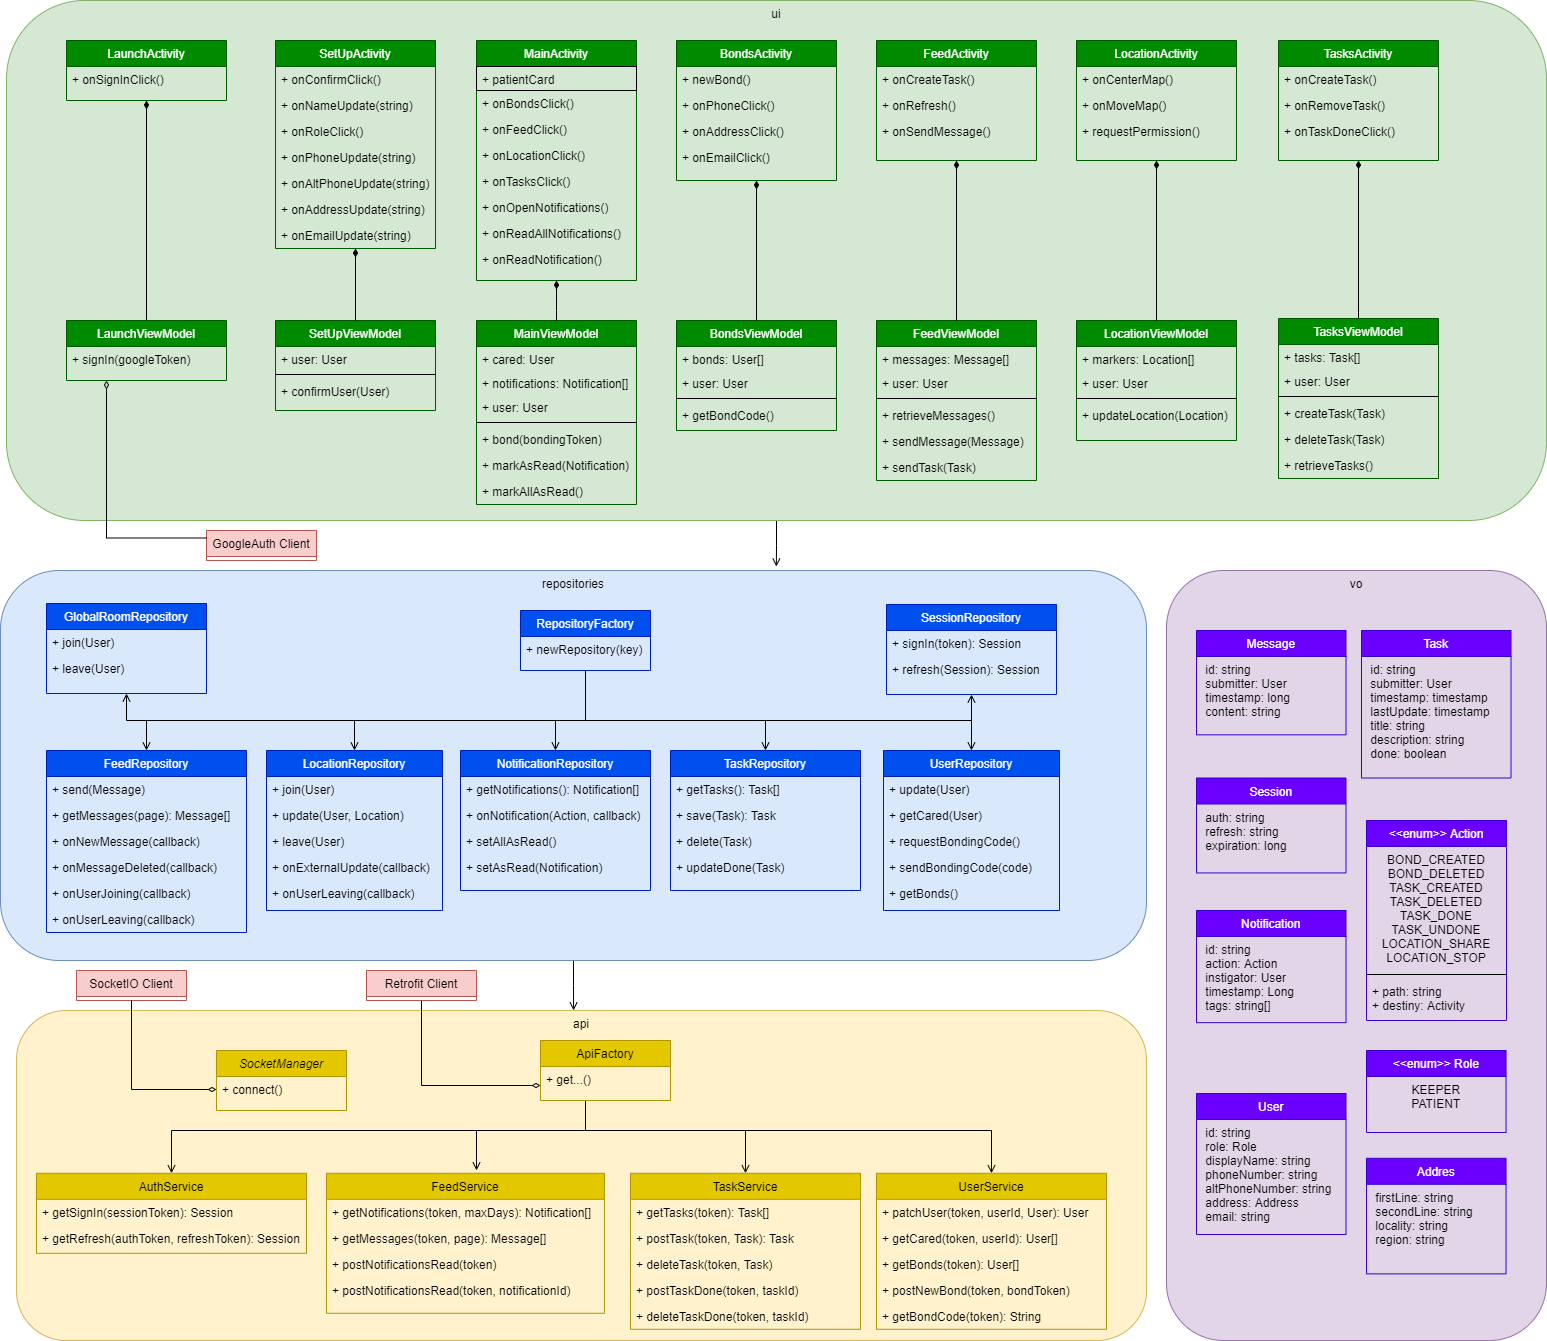
\includegraphics[width=1\textwidth]{images/Analisis/AnalisisDiagramaClasesApp.drawio.png}
    \caption{Diagrama de clases de la Aplicación}
    \label{fig:diagrama_clases_app}
\end{figure}

\subsection{UI}

\vspace{-5pt}
\subsubsection{Launch}

\begin{longtable}{|p{0.25\textwidth} p{0.75\textwidth}|}
    \hline
    \multicolumn{2}{|l|}{LaunchActivity} \\ \hline \hline
    Descripción      & Actividad de inicio de la aplicación con el inicio de sesión \\ \hline
    \multicolumn{2}{|l|}{Funciones} \\
    \emph{onSignClick}  & Arranca el proceso de inicio de sesión  \\ \hline
    \caption{Especificación de la clase LaunchActivity}
    \label{class:app:launch_activity}
\end{longtable}

\vspace{-15pt}
\begin{longtable}{|p{0.25\textwidth} p{0.75\textwidth}|}
    \hline
    \multicolumn{2}{|l|}{LaunchViewModel} \\ \hline \hline
    Descripción      & Modelo de la vista de LaunchActivity \\ \hline
    \multicolumn{2}{|l|}{Funciones} \\
    \emph{signIn}  & Solicita el inicio de sesión a la API  \\ \hline
    \caption{Especificación de la clase LaunchViewModel}
    \label{class:app:launch_view_model}
\end{longtable}

\vspace{-30pt}
\subsubsection{Set up}

\begin{longtable}{|p{0.25\textwidth} p{0.75\textwidth}|}
    \hline
    \multicolumn{2}{|l|}{SetUpActivity} \\ \hline \hline
    Descripción      & Actividad de configuración de la cuenta de usuario en la creación de esta \\ \hline
    \multicolumn{2}{|l|}{Funciones} \\
    \emph{onConfirmClick}  & Confirma la creación del usuario  \\
    \emph{onNameUpdate}  & Actualiza el nombre de usuario  \\ 
    \emph{onRoleClick}  & Selecciona un rol  \\ 
    \emph{onPhoneUpdate}  & Actualiza el número de teléfono principal \\
    \emph{onAltPhoneUpdate}  & Actualiza el número de teléfono alternativo  \\ 
    \emph{onAddressUpdate}  & Actualiza la dirección postal  \\ 
    \emph{onEmailUpdate}  & Actualiza la dirección electrónica  \\  \hline
    \caption{Especificación de la clase SetUpActivity}
    \label{class:app:setup_activity}
\end{longtable}

\vspace{-20pt}
\begin{longtable}{|p{0.25\textwidth} p{0.75\textwidth}|}
    \hline
    \multicolumn{2}{|l|}{SetUpViewModel} \\ \hline \hline
    Descripción      & Modelo de la vista de SetUpActivity \\ \hline
    \multicolumn{2}{|l|}{Propiedades} \\
    \emph{user}  & Información del usuario  \\ \hline
    \multicolumn{2}{|l|}{Funciones} \\
    \emph{confirmUser}  & Envía los datos del usuario para confirmarlo  \\ \hline
    \caption{Especificación de la clase SetUpViewModel}
    \label{class:app:setup_view_model}
\end{longtable}

\subsubsection{Main}

\vspace{-5pt}
\begin{longtable}{|p{0.3\textwidth} p{0.7\textwidth}|}
    \hline
    \multicolumn{2}{|l|}{MainActivity} \\ \hline \hline
    Descripción      & Actividad principal de la aplicación desde la que acceder a todas las funciones con la sesión iniciada \\ \hline
    \multicolumn{2}{|l|}{Propiedades} \\
    \emph{patientCard}  & Tarjeta con la información del Paciente vinculado (\ref{class:app:bonds_activity})  \\ \hline
    \multicolumn{2}{|l|}{Funciones} \\
    \emph{onBondsClick}  & Dirige al usuario a la actividad de vínculos (\ref{class:app:bonds_activity})  \\
    \emph{onFeedClick}  & Dirige al usuario a la actividad del feed (\ref{class:app:feed_activity})  \\ 
    \emph{onLocationClick}  & Dirige al usuario a la actividad de la geolocalización (\ref{class:app:feed_activity})  \\ 
    \emph{onTasksClick}  & Dirige al usuario a la actividad de gestión de tareas (\ref{class:app:tasks_activity})  \\ 
    \emph{onOpenNotifications}  & Despliega las notificaciones de usuario \\ 
    \emph{onReadAllNotifications}  & Marca todas las notificaciones como leídas \\ 
    \emph{onReadNotification}  & Marca una notificación como leída \\ \hline
    \caption{Especificación de la clase MainActivity}
    \label{class:app:main_activity}
\end{longtable}

\vspace{-20pt}
\begin{longtable}{|p{0.25\textwidth} p{0.75\textwidth}|}
    \hline
    \multicolumn{2}{|l|}{MainViewModel} \\ \hline \hline
    Descripción      & Modelo de la vista MainActivity \\ \hline
    \multicolumn{2}{|l|}{Propiedades} \\
    \emph{cared}  & Información del paciente vinculado  \\
    \emph{notifications}  & Lista de notificaciones no leídas del usuario  \\
    \emph{user}  & Información del usuario  \\ \hline
    \multicolumn{2}{|l|}{Funciones} \\
    \emph{bond}  & Envía una petición para crear un vínculo con otro usuario \\
    \emph{markAsRead}  & Envía una petición para marcar una notificación como leída \\ 
    \emph{markAsReadAll}  & Envía una petición para marcar todas las notificación como leída \\ \hline
    \caption{Especificación de la clase MainViewModel}
    \label{class:app:main_view_model}
\end{longtable}

\vspace{-30pt}
\subsubsection{Bonds}

\vspace{-5pt}
\begin{longtable}{|p{0.25\textwidth} p{0.75\textwidth}|}
    \hline
    \multicolumn{2}{|l|}{BondsActivity} \\ \hline \hline
    Descripción      & Actividad para la gestión de los vínculos \\ \hline
    \multicolumn{2}{|l|}{Funciones} \\
    \emph{newBond}  & Dirige al usuario a la actividad de vínculos  \\
    \emph{onPhoneClick}  & Abre la aplicación de teléfono con el número pulsado  \\ 
    \emph{onAddresClick}  & Abre la aplicación de mapas con la dirección pulsada \\ 
    \emph{onEmailClick}  & Abre la aplicación de correo electrónico con el email pulsado \\ \hline
    \caption{Especificación de la clase BondsActivity}
    \label{class:app:bonds_activity}
\end{longtable}

\begin{longtable}{|p{0.25\textwidth} p{0.75\textwidth}|}
    \hline
    \multicolumn{2}{|l|}{BondsViewModel} \\ \hline \hline
    Descripción      & Modelo de la vista BondsActivity \\ \hline
    \multicolumn{2}{|l|}{Propiedades} \\
    \emph{bonds}  & Lista con la información de los usuarios asociados  \\
    \emph{user}  & Información del usuario  \\ \hline
    \multicolumn{2}{|l|}{Funciones} \\
    \emph{getBondCode}  & Envía una petición para obtener un token de vinculación \\ \hline
    \caption{Especificación de la clase BondsViewModel}
    \label{class:app:bonds_view_model}
\end{longtable}

\vspace{-32pt}
\subsubsection{Feed}

\vspace{-7pt}
\begin{longtable}{|p{0.25\textwidth} p{0.75\textwidth}|}
    \hline
    \multicolumn{2}{|l|}{FeedActivity} \\ \hline \hline
    Descripción      & Actividad de la aplicación con el chat entre usuarios asociados \\ \hline
    \multicolumn{2}{|l|}{Funciones} \\
    \emph{onCreateTask}  & Envía el mensaje como tarea \\
    \emph{onRefresh}  & Actualiza la lista de mensajes  \\ 
    \emph{onSendMessage}  & Envía el mensaje  \\ \hline
    \caption{Especificación de la clase FeedActivity}
    \label{class:app:feed_activity}
\end{longtable}

\vspace{-22pt}
\begin{longtable}{|p{0.25\textwidth} p{0.75\textwidth}|}
    \hline
    \multicolumn{2}{|l|}{FeedViewModel} \\ \hline \hline
    Descripción      & Modelo de la vista FeedActivity \\ \hline
    \multicolumn{2}{|l|}{Propiedades} \\
    \emph{messages}  & Lista con los mensajes del Feed  \\
    \emph{user}  & Información del usuario  \\ \hline
    \multicolumn{2}{|l|}{Funciones} \\
    \emph{retrieveMessage}  & Envía una petición para recuperar los mensajes \\
    \emph{sendMessage}  & Envía el mensaje al resto de usuarios \\
    \emph{sendTask}  & Envía la tarea al resto de usuarios \\ \hline
    \caption{Especificación de la clase FeedViewModel}
    \label{class:app:feed_view_model}
\end{longtable}

\vspace{-32pt}
\subsubsection{Location}

\vspace{-7pt}
\begin{longtable}{|p{0.25\textwidth} p{0.75\textwidth}|}
    \hline
    \multicolumn{2}{|l|}{LocationActivity} \\ \hline \hline
    Descripción      & Actividad con el mapa de la geolocalización \\ \hline
    \multicolumn{2}{|l|}{Funciones} \\
    \emph{onCenterMap}  & Centra el mapa en el usuario  \\
    \emph{onMoveMap}  & Mueve el mapa  \\ 
    \emph{requestPermission}  & Solicita el permiso del usuario para usar la geolocalización  \\ \hline
    \caption{Especificación de la clase LocationActivity}
    \label{class:app:location_activity}
\end{longtable}

\begin{longtable}{|p{0.25\textwidth} p{0.75\textwidth}|}
    \hline
    \multicolumn{2}{|l|}{LocationViewModel} \\ \hline \hline
    Descripción      & Modelo de la vista LocationActivity \\ \hline
    \multicolumn{2}{|l|}{Propiedades} \\
    \emph{markers}  & Lista de localizaciones del resto de usuarios  \\
    \emph{user}  & Información del usuario  \\ \hline
    \multicolumn{2}{|l|}{Funciones} \\
    \emph{updateLocation}  & Envía la localización al resto de usuarios \\ \hline
    \caption{Especificación de la clase LocationViewModel}
    \label{class:app:location_view_model}
\end{longtable}

\vspace{-31pt}
\subsubsection{Tasks}

\vspace{-21pt}
\begin{figure}[H]
\begin{longtable}{|p{0.25\textwidth} p{0.75\textwidth}|}
    \hline
    \multicolumn{2}{|l|}{TasksActivity} \\ \hline \hline
    Descripción      & Actividad para la gestión de tareas \\ \hline
    \multicolumn{2}{|l|}{Funciones} \\
    \emph{onCreateTask}  & Confirma la creación de una tarea \\
    \emph{onRemoveTask}  & Elimina una tarea  \\ 
    \emph{onTaskDoneClick}  & Cambia el estado de una tarea  \\ \hline
    \caption{Especificación de la clase TasksActivity}
    \label{class:app:tasks_activity}
\end{longtable}
\end{figure}

\vspace{-21pt}
\begin{longtable}{|p{0.25\textwidth} p{0.75\textwidth}|}
    \hline
    \multicolumn{2}{|l|}{TasksViewModel} \\ \hline \hline
    Descripción      & Modelo de la vista TasksActivity \\ \hline
    \multicolumn{2}{|l|}{Propiedades} \\
    \emph{tasks}  & Lista de tareas relevantes del usuario  \\
    \emph{user}  & Información del usuario  \\ \hline
    \multicolumn{2}{|l|}{Funciones} \\
    \emph{createTask}  & Envía una nueva tarea para crear \\
    \emph{deleteTask}  & Envía una petición para eliminar una tarea \\
    \emph{retrieveTasks}  & Recupera la lista de tareas relevantes del usuario \\ \hline
    \caption{Especificación de la clase TasksViewModel}
    \label{class:app:tasks_view_model}
\end{longtable}

\vspace{-36pt}
\subsection{Repositories}

\vspace{-11pt}
\subsubsection{RepositoryFactory}

\begin{longtable}{|p{0.25\textwidth} p{0.75\textwidth}|}
    \hline
    \multicolumn{2}{|l|}{RepositoryFactory} \\ \hline \hline
    Descripción      & Factoría de repositorios \\ \hline
    \multicolumn{2}{|l|}{Funciones} \\
    \emph{newRepository}  & Genera y devuelve el repositorio solicitado \\ \hline
    \caption{Especificación de la clase RepositoryFactory}
    \label{class:app:repository_factory}
\end{longtable}

\subsubsection{FeedRepository}

\begin{longtable}{|p{0.25\textwidth} p{0.75\textwidth}|}
    \hline
    \multicolumn{2}{|l|}{FeedRepository} \\ \hline \hline
    Descripción      & Repositorio para la gestión de las operaciones relacionadas con el feed \\ \hline
    \multicolumn{2}{|l|}{Funciones} \\
    \emph{send}  & Envía un mensaje \\
    \emph{getMessages}  & Recupera la lista de mensajes \\
    \emph{onNewMessage}  & Suscribe una acción a la entrada de un nuevo mensaje \\
    \emph{onMessageDeleted}  & Suscribe una acción a la eliminación de un mensaje \\
    \emph{onUserJoining}  & Suscribe una acción a la conexión de un usuario a la sala del feed \\
    \emph{onUserLeaving}  & Suscribe una acción a la desconexión de un usuario a la sala del feed \\ \hline
    \caption{Especificación de la clase FeedRepository}
    \label{class:app:feed_repository}
\end{longtable}

\subsubsection{GlobalRoomRepository}

\begin{longtable}{|p{0.25\textwidth} p{0.75\textwidth}|}
    \hline
    \multicolumn{2}{|l|}{GlobalRoomRepository} \\ \hline \hline
    Descripción      & Repositorio para la gestión de la conexión con la sala Global \\ \hline
    \multicolumn{2}{|l|}{Funciones} \\
    \emph{join}  & Conecta al usuario a la sala Global \\
    \emph{leave}  & Desconecta al usuario de la sala Global \\ \hline
    \caption{Especificación de la clase GlobalRoomRepository}
    \label{class:app:global_room_repository}
\end{longtable}

\subsubsection{LocationRepository}

\begin{longtable}{|p{0.25\textwidth} p{0.75\textwidth}|}
    \hline
    \multicolumn{2}{|l|}{LocationRepository} \\ \hline \hline
    Descripción      & Repositorio para operaciones relacionadas con la geolocalización \\ \hline
    \multicolumn{2}{|l|}{Funciones} \\
    \emph{join}  & Suscribe al usuario a la sala de geolocalización \\
    \emph{update}  & Actualiza la localización del usuario \\
    \emph{leave}  & Desconecta al usuario de la sala de geolocalización \\
    \emph{onExternalUpdate}  & Suscribe una acción a la llegada de actualizaciones \\
    \emph{onUserLeaving}  & Suscribe una acción a la desconexión de un usuario \\ \hline
    \caption{Especificación de la clase LocationRepository}
    \label{class:app:location_repository}
\end{longtable}

\subsubsection{NotificationRepository}

\begin{longtable}{|p{0.25\textwidth} p{0.75\textwidth}|}
    \hline
    \multicolumn{2}{|l|}{NotificationRepository} \\ \hline \hline
    Descripción      & Repositorio para operaciones relacionadas con las notificaciones \\ \hline
    \multicolumn{2}{|l|}{Funciones} \\
    \emph{getNotifications}  & Recupera la lista de notificaciones \\
    \emph{onNotification}  & Suscribe una acción a la llegada de una nueva notificación \\
    \emph{setAllAsRead}  & Marca todas las notificaciones como leídas \\
    \emph{setAsRead}  & Marca una notificación como leída \\ \hline
    \caption{Especificación de la clase NotificationRepository}
    \label{class:app:notification_repository}
\end{longtable}

\subsubsection{SessionRepository}

\begin{longtable}{|p{0.25\textwidth} p{0.75\textwidth}|}
    \hline
    \multicolumn{2}{|l|}{SessionRepository} \\ \hline \hline
    Descripción      & Repositorio para operaciones relacionadas con la sesión \\ \hline
    \multicolumn{2}{|l|}{Funciones} \\
    \emph{signIn}  & Inicia la sesión del usuario \\
    \emph{refresh}  & Refresca la sesión del usuario \\ \hline
    \caption{Especificación de la clase SessionRepository}
    \label{class:app:session_repository}
\end{longtable}

\subsubsection{TasksRepository}

\begin{longtable}{|p{0.25\textwidth} p{0.75\textwidth}|}
    \hline
    \multicolumn{2}{|l|}{TasksRepository} \\ \hline \hline
    Descripción      & Repositorio para operaciones relacionadas con las tareas \\ \hline
    \multicolumn{2}{|l|}{Funciones} \\
    \emph{delete}  & Elimina una tarea \\
    \emph{getTasks}  & Recupera las tareas \\
    \emph{save}  & Guarda una tarea \\
    \emph{update}  & Actualiza una tarea \\ \hline
    \caption{Especificación de la clase TasksRepository}
    \label{class:app:tasks_repository}
\end{longtable}

\newpage
\subsubsection{UserRepository}

\begin{longtable}{|p{0.25\textwidth} p{0.75\textwidth}|}
    \hline
    \multicolumn{2}{|l|}{UserRepository} \\ \hline \hline
    Descripción      & Repositorio para operaciones relacionadas con los usuarios \\ \hline
    \multicolumn{2}{|l|}{Funciones} \\
    \emph{update}  & Actualiza los datos del usuario \\
    \emph{getCared}  & Recupera los datos del Paciente vinculado \\
    \emph{requestBondingCode}  & Solicita un token de vinculación \\
    \emph{sendBondingCode}  & Elimina un token de vinculación \\
    \emph{getBonds}  & Recupera los vínculos del usuario \\ \hline
    \caption{Especificación de la clase UserRepository}
    \label{class:app:user_repository}
\end{longtable}

\vspace{-30pt}
\subsection{API}

\vspace{-10pt}
\subsubsection{ApiFactory}

\begin{longtable}{|p{0.25\textwidth} p{0.75\textwidth}|}
    \hline
    \multicolumn{2}{|l|}{ApiFactory} \\ \hline \hline
    Descripción      & Factoría de servicios de la API \\ \hline
    \multicolumn{2}{|l|}{Funciones} \\
    \emph{get}  & Crea y regresa el servicio solicitado \\ \hline
    \caption{Especificación de la clase ApiFactory}
    \label{class:app:api_factory}
\end{longtable}

\vspace{-20pt}
\subsubsection{SocketManager}

\begin{longtable}{|p{0.25\textwidth} p{0.75\textwidth}|}
    \hline
    \multicolumn{2}{|l|}{SocketManager} \\ \hline \hline
    Descripción      & Clase a cargo de la gestión del socket \\ \hline
    \multicolumn{2}{|l|}{Funciones} \\
    \emph{connect}  & Conecta al usuario a la API WebSocket \\ \hline
    \caption{Especificación de la clase SocketManager}
    \label{class:app:socket_manager}
\end{longtable}

\vspace{-20pt}
\subsubsection{AuthService}

\begin{longtable}{|p{0.25\textwidth} p{0.75\textwidth}|}
    \hline
    \multicolumn{2}{|l|}{AuthService} \\ \hline \hline
    Descripción      & Servicio para la realización de peticiones al endpoint /auth \\ \hline
    \multicolumn{2}{|l|}{Funciones} \\
    \emph{getSignIn}  & Realiza una petición a GET /auth/signin \\
    \emph{getRefresh}  & Realiza una petición a GET /auth/refresh \\ \hline
    \caption{Especificación de la clase AuthService}
    \label{class:app:auth_service}
\end{longtable}

\subsubsection{FeedService}

\begin{longtable}{|p{0.25\textwidth} p{0.75\textwidth}|}
    \hline
    \multicolumn{2}{|l|}{FeedService} \\ \hline \hline
    Descripción      & Servicio para la realización de peticiones al endpoint /feed \\ \hline
    \multicolumn{2}{|l|}{Funciones} \\
    \emph{getNotifications}  & Realiza una petición a GET /feed/notification \\
    \emph{getMessages}  & Realiza una petición a GET /feed/message \\
    \emph{postNotificationsRead}  & Realiza una petición a POST /feed/notification/read \\  \hline
    \caption{Especificación de la clase FeedService}
    \label{class:app:feed_service}
\end{longtable}

\subsubsection{TaskService}

\begin{longtable}{|p{0.25\textwidth} p{0.75\textwidth}|}
    \hline
    \multicolumn{2}{|l|}{TaskService} \\ \hline \hline
    Descripción      & Servicio para la realización de peticiones al endpoint /task \\ \hline
    \multicolumn{2}{|l|}{Funciones} \\
    \emph{getTasks}  & Realiza una petición a GET /task \\
    \emph{postTask}  & Realiza una petición a POST /task \\
    \emph{deleteTask}  & Realiza una petición a DELETE /task \\
    \emph{postTaskDone}  & Realiza una petición a POST /task/done \\
    \emph{deleteTaskDone}  & Realiza una petición a DELETE /task/done \\  \hline
    \caption{Especificación de la clase TaskService}
    \label{class:app:task_service}
\end{longtable}

\subsubsection{UserService}

\begin{longtable}{|p{0.25\textwidth} p{0.75\textwidth}|}
    \hline
    \multicolumn{2}{|l|}{UserService} \\ \hline \hline
    Descripción      & Servicio para la realización de peticiones al endpoint /user \\ \hline
    \multicolumn{2}{|l|}{Funciones} \\
    \emph{patchUser}  & Realiza una petición a PATCH /user \\
    \emph{getCared}  & Realiza una petición a GET /user/bond/cared \\
    \emph{getBonds}  & Realiza una petición a GET /user/bond \\
    \emph{postNewBond}  & Realiza una petición a POST /user/bond \\
    \emph{getBondCode}  & Realiza una petición a GET /user/bond \\  \hline
    \caption{Especificación de la clase UserService}
    \label{class:app:user_service}
\end{longtable}

\subsection{VO}

\subsubsection{Message}

\begin{longtable}{|p{0.25\textwidth} p{0.75\textwidth}|}
    \hline
    \multicolumn{2}{|l|}{Message} \\ \hline \hline
    Descripción      & Objeto representante de un mensaje \\ \hline
    \multicolumn{2}{|l|}{Propiedades} \\
    \emph{id}  & Identidad del mensaje \\
    \emph{submitter}  & Usuario que envió el mensaje \\
    \emph{timestamp}  & Instante de creación del mensaje \\
    \emph{content}  & Contenido del mensaje \\  \hline
    \caption{Especificación de la clase Message de la aplicación}
    \label{class:app:message}
\end{longtable}

\subsubsection{Task}

\begin{longtable}{|p{0.25\textwidth} p{0.75\textwidth}|}
    \hline
    \multicolumn{2}{|l|}{Task} \\ \hline \hline
    Descripción      & Objeto representante de una tarea \\ \hline
    \multicolumn{2}{|l|}{Propiedades} \\
    \emph{id}  & ID \\
    \emph{submitter}  & Usuario que envió la tarea \\
    \emph{timestamp}  & Instante de creación del mensaje \\
    \emph{lastUpdate}  & Instante de última actualización del mensaje \\
    \emph{title}  & Título \\
    \emph{description}  & Descripción \\
    \emph{done}  & Estado: hecha o no hecha \\  \hline
    \caption{Especificación de la clase Task de la aplicación}
    \label{class:app:task}
\end{longtable}

\subsubsection{Session}

\begin{longtable}{|p{0.25\textwidth} p{0.75\textwidth}|}
    \hline
    \multicolumn{2}{|l|}{Session} \\ \hline \hline
    Descripción      & Objeto representante de una sesión \\ \hline
    \multicolumn{2}{|l|}{Propiedades} \\
    \emph{auth}  & Token de autenticación \\
    \emph{refresh}  & Token de refresco \\
    \emph{expiration}  & Instante de expiración de la sesión \\  \hline
    \caption{Especificación de la clase Session de la aplicación}
    \label{class:app:session}
\end{longtable}

\subsubsection{Notification}

\begin{longtable}{|p{0.25\textwidth} p{0.75\textwidth}|}
    \hline
    \multicolumn{2}{|l|}{Notification} \\ \hline \hline
    Descripción      & Objeto representante de una notificación \\ \hline
    \multicolumn{2}{|l|}{Propiedades} \\
    \emph{id}  & ID \\
    \emph{action}  & Acción notificada \\
    \emph{instigator} & Usuario que realizó la acción \\
    \emph{timestamp}  & Instante de creación de la notificación \\
    \emph{tags}  & Etiquetas de la notificación \\  \hline
    \caption{Especificación de la clase Notification de la aplicación}
    \label{class:app:notification}
\end{longtable}

\begin{longtable}{|p{0.25\textwidth} p{0.75\textwidth}|}
    \hline
    \multicolumn{2}{|l|}{Action} \\ \hline \hline
    Descripción      & Lista de acciones notificables \\ \hline
    \multicolumn{2}{|l|}{Valores} \\
    \emph{BOND CREATED}  & Creación de un vínculo  \\
    \emph{BOND DELETED}  & Eliminación de un vínculo  \\
    \emph{TASK CREATED}  & Creación de una tarea  \\
    \emph{TASK DELETED}  & Eliminación de una tarea  \\
    \emph{TASK DONE}  & Actualización de una tarea a hecha  \\
    \emph{TASK UNDONE}  & Actualización de una tarea a no hecha  \\
    \emph{LOCATION SHARE}  & Ubicación empezando a ser compartida  \\
    \emph{LOCATION STOP}  & Ubicación dejando de ser compartida  \\ \hline
    \multicolumn{2}{|l|}{Propiedades} \\
    \emph{path}  & Ruta de la notificación \\
    \emph{destiny}  & Actividad destino si la tiene \\  \hline
    \caption{Especificación de la clase Action de la aplicación}
    \label{class:app:action}
\end{longtable}

\newpage
\subsubsection{User}

\begin{longtable}{|p{0.25\textwidth} p{0.75\textwidth}|}
    \hline
    \multicolumn{2}{|l|}{User} \\ \hline \hline
    Descripción      & Objeto representante de un usuario \\ \hline
    \multicolumn{2}{|l|}{Propiedades} \\
    \emph{id}  & ID \\
    \emph{role}  & Rol \\
    \emph{displayName}  & Nombre visible \\
    \emph{phoneNumber}  & Número de teléfono \\
    \emph{altPhoneNumber}  & Número alternativo de teléfono \\
    \emph{address}  & Dirección postal \\
    \emph{email}  & Dirección electrónica \\  \hline
    \caption{Especificación de la clase User de la aplicación}
    \label{class:app:user}
\end{longtable}

\begin{longtable}{|p{0.25\textwidth} p{0.75\textwidth}|}
    \hline
    \multicolumn{2}{|l|}{Role} \\ \hline \hline
    Descripción      & Lista de posibles roles de los usuarios \\ \hline
    \multicolumn{2}{|l|}{Valores} \\
    \emph{PATIENT}  & Pacientes  \\
    \emph{KEEPER}  & Cuidadores  \\ \hline
    \caption{Especificación de la clase Role de la aplicación}
    \label{class:app:role}
\end{longtable}

\begin{longtable}{|p{0.25\textwidth} p{0.75\textwidth}|}
    \hline
    \multicolumn{2}{|l|}{Address} \\ \hline \hline
    Descripción      & Objeto representante de una dirección postal \\ \hline
    \multicolumn{2}{|l|}{Propiedades} \\
    \emph{firstLine}  & Primera línea \\
    \emph{secondLine}  & Segunda línea \\
    \emph{locality}  & Localidad \\
    \emph{region}  & Región \\  \hline
    \caption{Especificación de la clase Address de la aplicación}
    \label{class:app:address}
\end{longtable}